\subsection{Turret design}
% Maybe add a note here that the turret is mostly designed for you, but you evaluated a design excursion to look at a motor sized for X requirements. Also this kind of needs a picture with callouts. 

To determine the motor requirements, we first defined the desired response of the motor. Then, we computed a rough estimate of the moment of inertia using the mass and geometry of various parts of the turret system. This allowed us to determine what torque would be necessary to drive the motor according to our specifications. (put spreadsheet in appendix on overleaf).

We chose a motor that could fulfil all the desired requirements. Both motors on the decision tree met requirements, so to reduce costs, we chose the motor that exceeded the requisites by less. Our final choice of motor, the MATSUSHITA PN GMX-6MP009A is the one already employed in the turret, our decision simply confirmed this was the right choice. 

Motor torque, speed, and current information was all available from the data sheet on the robotics and controls website. (Currently unavailable, will create plots once get data).

The turret motor is controlled by the mbed and a TD340 motor driver. The motor requires higher voltage and current than the mbed can supply, leading to the intermediary. The mbed supplies two signals, a digital out for direction, and a pwm signal for speed. We chose to use pwm from the mbed instead of analog out because the analog signal requires two conversions, increasing chances for error. The analog and digital speed control use two different input pins on the motor driver. A pulldown resistor had to be placed on the speed control pin to prevent the system actuating on startup. The connection to ground reduced the effect of noise on the system.
\begin{figure}[h]
    \centering
    \includegraphics[scale=.4]{pos mot data.png}
    \caption{Positive Motion Data}
    \label{fig:pos mot}
\end{figure}
\begin{figure}[h]
    \centering
    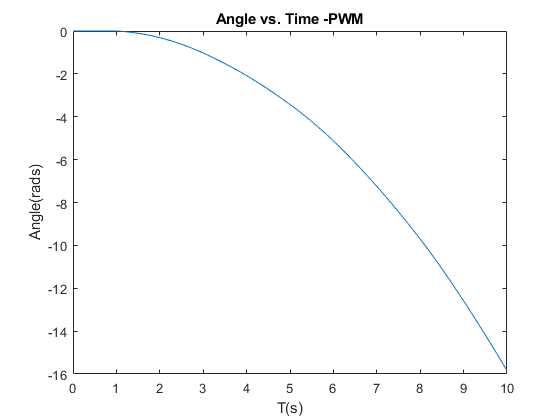
\includegraphics[scale=.4]{neg mot data.png}
    \caption{Negative Motion Data}
    \label{fig:neg mot data}
\end{figure}
D: To change the turret direction, the mbed digital out is changed from high to low. While the turret has the same internal mechanics both directions, the difference in signs leads to two separate transfer functions and models. Positive rotation: 5.9169/(s+0.4674) (s+0.01372) 
Negative rotation: 0.89934/(s+0.02155) (s+0.0289)

 \begin{figure}[h!]
     \centering
     \includegraphics[scale=.3]{tfPos.jpg}
     \caption{Turret's Positive Transfer Function}
     \label{fig:postf}
 \end{figure}
 \begin{figure}[h!]
     \centering
     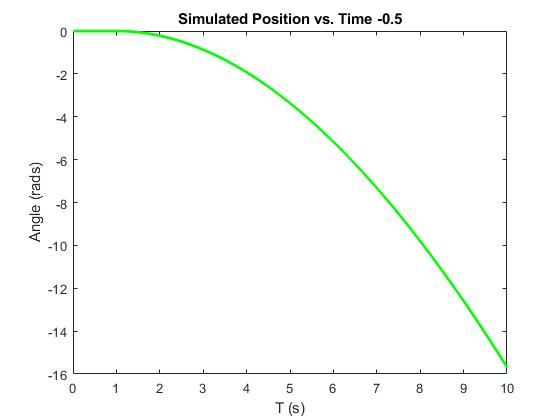
\includegraphics[scale=.3]{tfNeg.jpg}
     \caption{Turret's Negative Transfer Function }
     \label{fig:negtf}
 \end{figure}                             
                          
 
